% vim:set textwidth=100:
% vim:set fo+=t:

\documentclass[12pt]{article}

\usepackage{amsmath}
\usepackage[nofiglist,notablist]{endfloat}
\usepackage[usenames,dvipsnames]{color}
\usepackage{color}
\usepackage{authblk}
\usepackage{graphicx}
\usepackage{palatino}
\usepackage[activate={true,nocompatibility},final]{microtype}
\usepackage[super,sort&compress]{natbib}
\pagenumbering{arabic}
\parskip = 0.08in \parindent = 0.0in

% Custom macros for author comments
\newcommand{\Alberto}[1]{\color{ForestGreen}#1\normalcolor }
\newcommand{\Justin}[1]{\color{blue}#1\normalcolor}
\newcommand{\Arijit}[1]{\color{magenta}#1\normalcolor}
\newcommand{\Ken}[1]{\color{red}#1\normalcolor}

\author{Arijit~Roy}
\author{Alberto~Perez}
\author{Ken~A.~Dill}
\author{Justin~L.~MacCallum}
\affil{Laufer Center for Physical and Quantitative Biology\\
    and Departments of Physics and Chemistry\\
    Stony Brook University\\
    Stony Brook, NY 11794-5252.}

\title{Predicting the conformational preferences of proteins using a physics-based free energy
method}

\begin{document}

\maketitle


\section*{Preparation of input models for chamelon sequences}

We prepared computer generated models in both $\alpha$ and $\beta$ conformations for all five chamelon sequences mentioned 
in the main text. The crystallographic structure of GA95 and GB95 sequences have $\alpha$ and $\beta$ fold respectively.
To prepare the $\alpha$ and $\beta$ fold for the GA95 sequence, we start with the crystallographic
conformation of the native GA95 and GB95 sequences. 
We then remove the sidechains at three mutated positions in both folds
and call the program SCWRL4 \cite{Krivov2009} to generate the side chain conformations of the
mutated residues and their neighbors. Followed by 
this step, we perform extensive molecular dynamics
minimizations to remove any possible bad contact. This procedure was used to generate all $\alpha$ and 
$\beta$ conformations for the five sequences that were used in the free energy calculation.   

\setcounter{figure}{0}
\makeatletter 
\renewcommand{\thefigure}{S\@arabic\c@figure}
\begin{figure}
\includegraphics[width=5.6 in,height=5.3 in]{orban_perres_SI.pdf}
\label{fig:orban_full}
\caption{Per residue free energy calculations indicate significant differences of side chain orientation of key amino acid residues. These amino acid
residues displace the free energy equilibrium to either $\beta$ or
$\alpha$ conformation. All figures in the left are in $\beta$ conformation, whereas the right ones are in $\alpha$ conformation except in Figure (F) 
where both are in $\alpha$ conformation.
Sidechains of hydrophobic residues L7 in (A) and A26 in (B) are oriented towards the protein interior in $\beta$ 
conformation. In such conformation they have hydrophobic interactions with other hydrophobic residues colored in white. In $\alpha$ conformation these residues are 
exposed to the protein surface.  
(C) Y45 forms H-bond with D47 with GB95 sequence and $\beta$ conformation. (D) Q11 and E15 forms a salt bridge in $\beta$ conformation which is absent
in the $\alpha$ conformation. (E) Hydrophobic I49 is exposed to the protein surface in $\beta$ conformation, whereas in $\alpha$ conformation it 
is inside protein hydrophobic core. (F) Sidechain of I30 is inside the protein hydrophobic core as it has a smaller sidechain with GA95 sequence 
and $\alpha$ conformation. In contrast, Phe-30 with larger sidechain is exposed to the protein surface with GB95 sequence and $\beta$ conformation.}
\end{figure}

\begin{figure}
    \begin{center}
        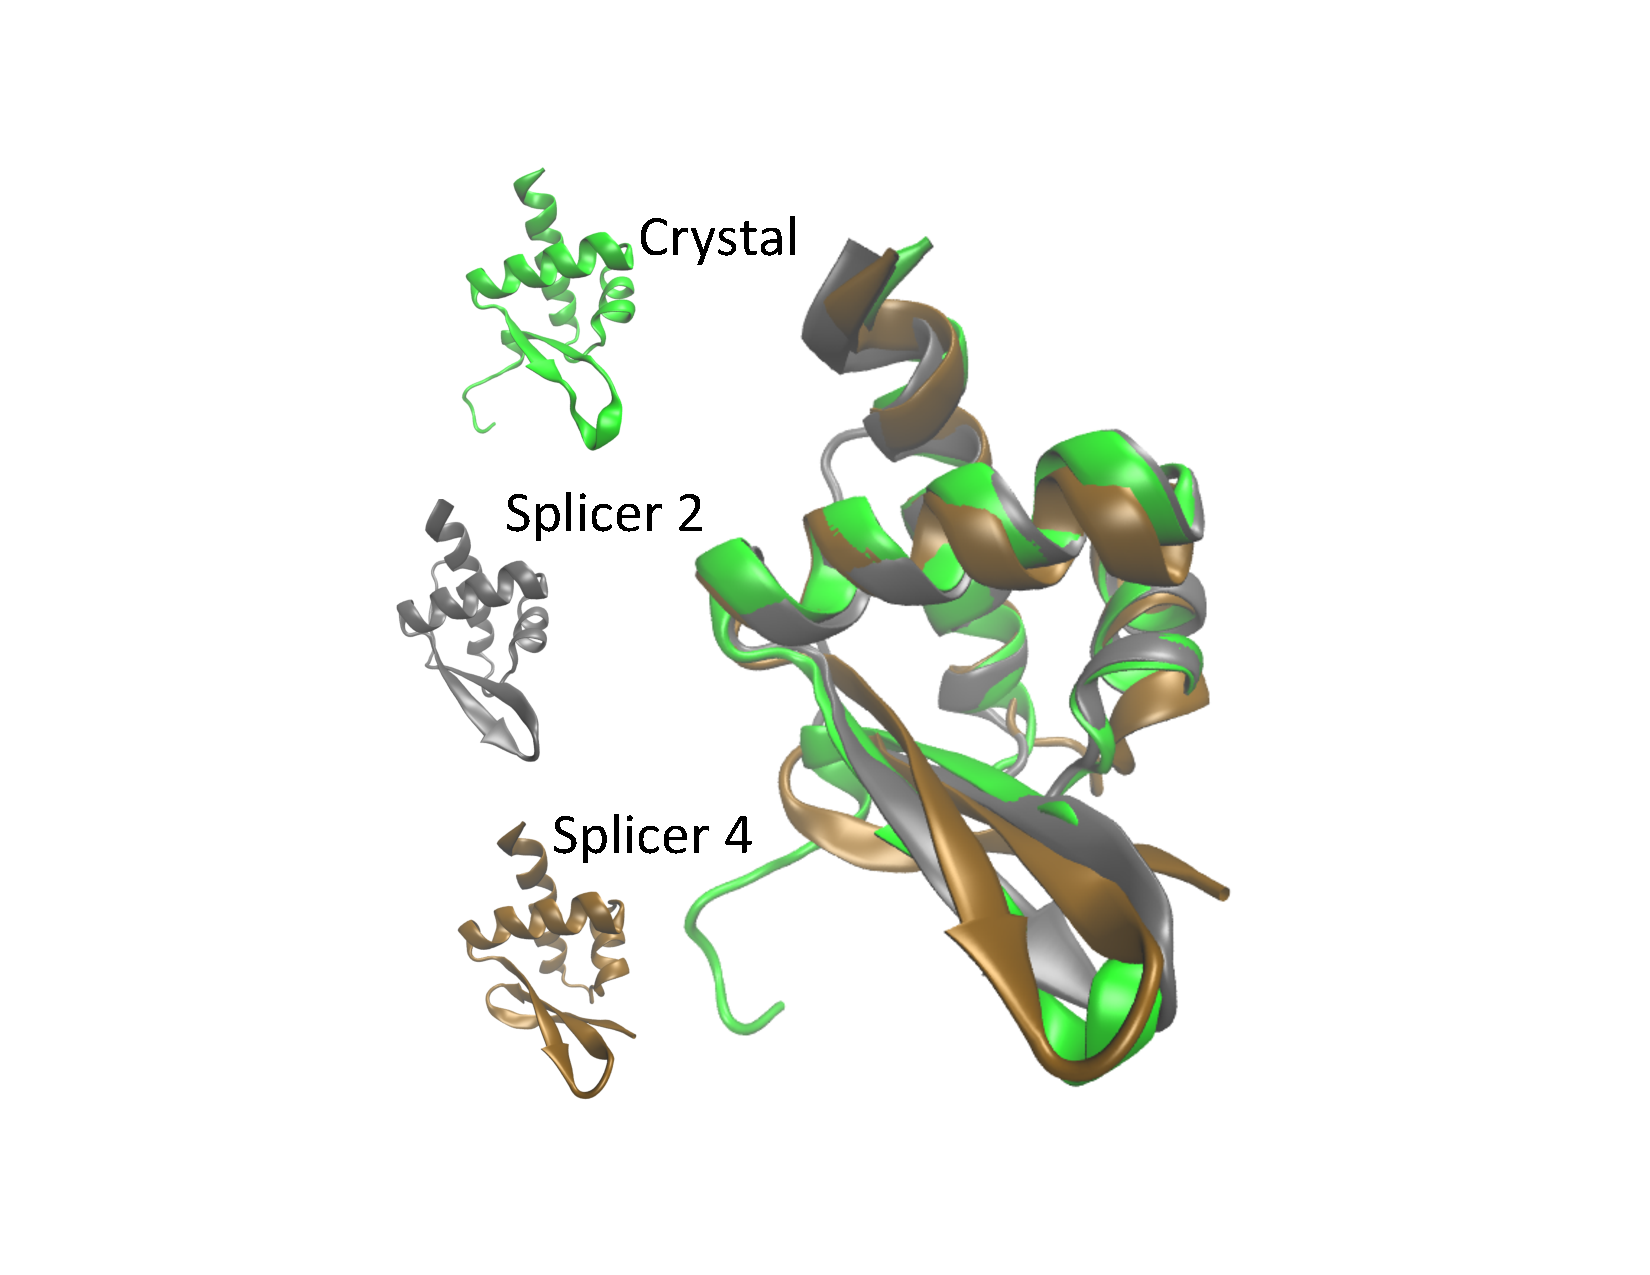
\includegraphics[width=3.5 in]{T0560.pdf}
    \end{center}
    \caption{Native structure and two models (from group ``Splicer'') for target T0560.}
    \label{fig:T0560}
\end{figure}


\begin{figure}
\begin{center}
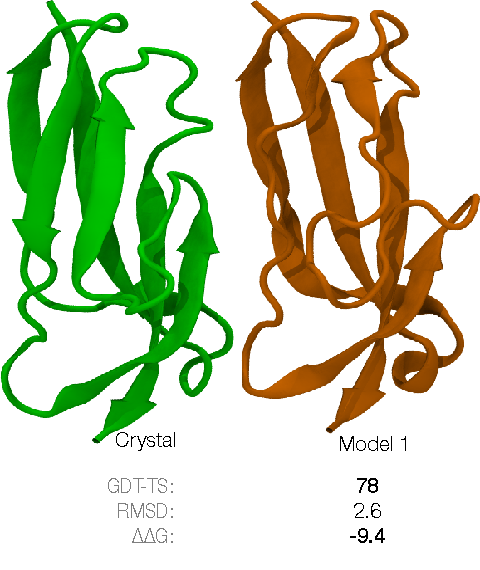
\includegraphics[width=3.8 in,height=3.4 in]{T0569.pdf}
\end{center}
\caption{Native and best computer generated model structure of CASP Target T0569.} 
\label{fig:T0569}
\end{figure}


\begin{figure}
\begin{center}
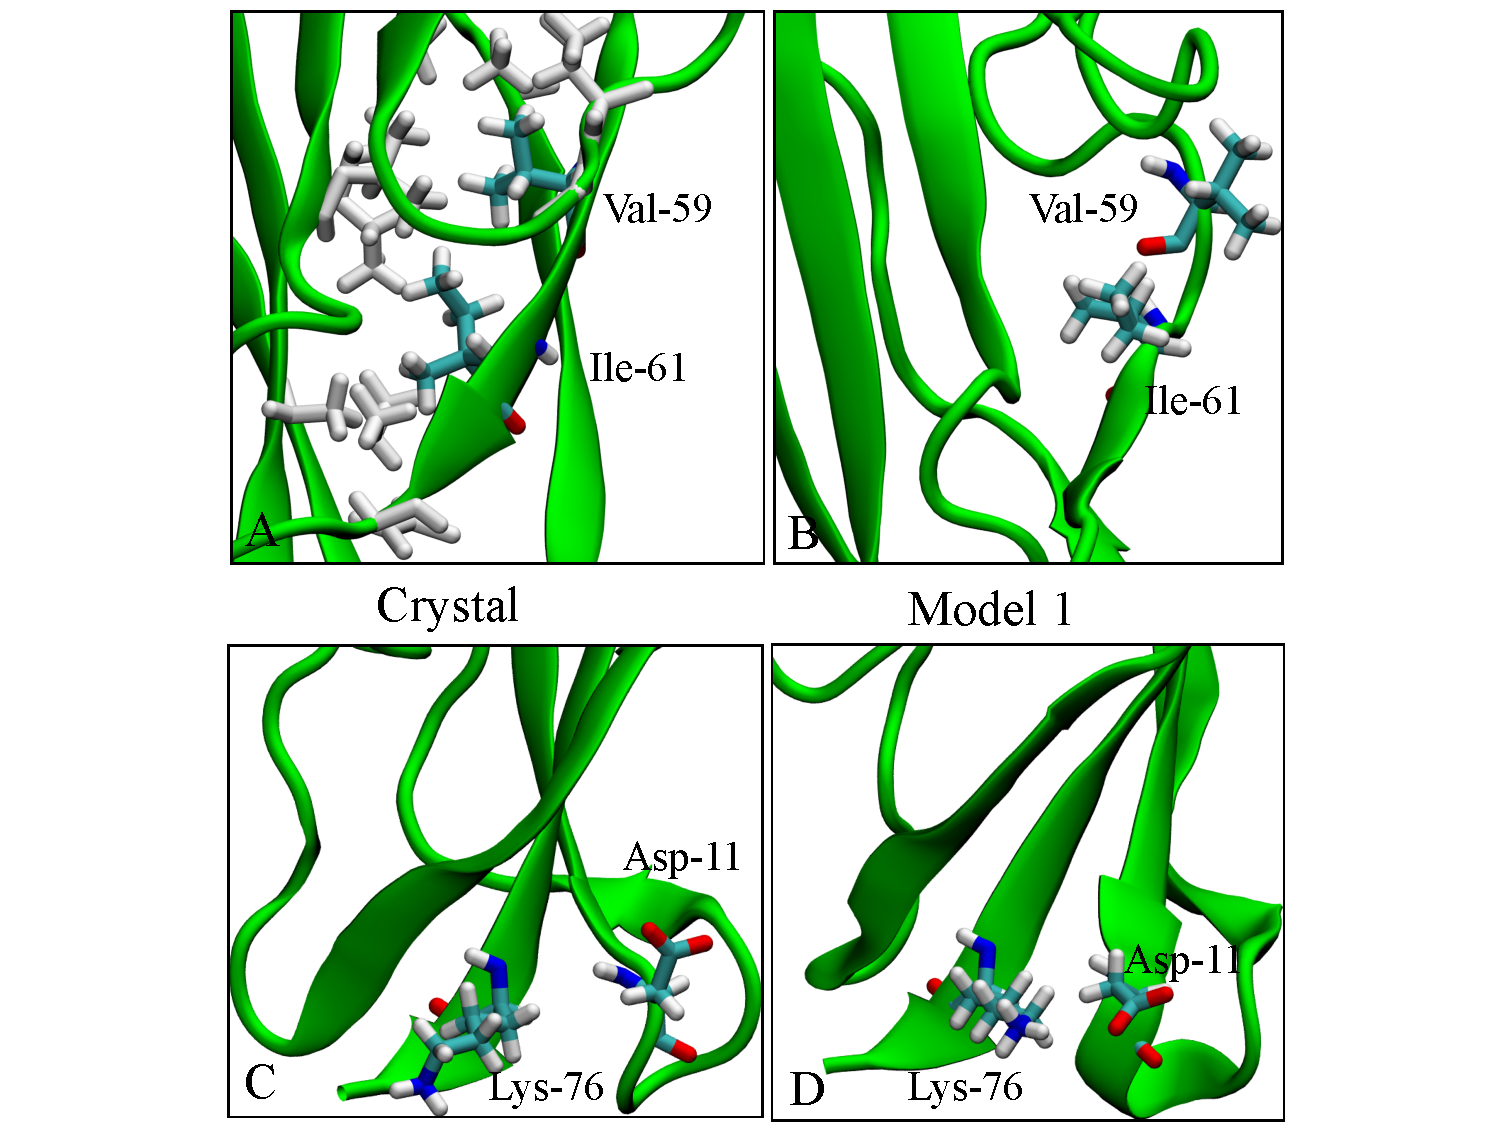
\includegraphics[width=5 in,height=4 in]{T0569_perres2.pdf}
\end{center}
\caption{Key differences between the experimental structure and the computer generated models as
    indicated by the per residue free energy calculation.
The side chains of hydrophobic residues, V59 and I61 are oriented towards the protein hydrophobic core in (A)  
, in (B) they are exposed to the surface. The beta sheet containing these residues is disordered in
the generated model due to
a salt bridge between K76 and D11 in (D) the computer generated structure, which is absent in the (C) native structure.}
\label{fig:T0569_per_residue}
\end{figure}

\begin{figure}
\begin{center}
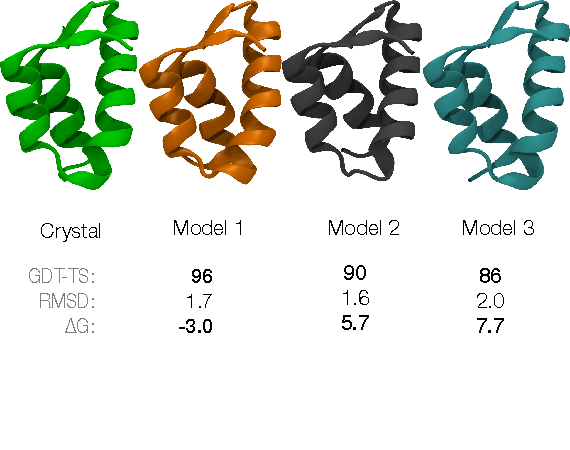
\includegraphics[width=3.5in]{T0538.pdf}
\end{center}
\caption{The free energy based ranking of the experimental and three predicted structures for an engineered protein (PDB ID: 2L09 and CASP
    code:T0538). Models 1,2 and 3 are from the group PconsR, Shell and FOLDIT respectively. In this case, one of the predicted structure 
    was found to be more stable than the experimental strucre.}
\label{fig:T0538}
\end{figure}


\section*{What can we say about low resolution models from CASP experiments?}

In the main text, we discussed how well confinement method predicted preferences when the structures are not very far from the
native. But the question remains how far from native can we go and still see that the method produces correct result. In
this section we explored this question with models from the extracellular domain of the jumping translocation breakpoint
protein (pdb id: 2KJX). Most of the groups could only generate low resolution models for this CASP9 target (id: T0531).
In our comparison, we chose five models by the MUFOLD-MD group, which was the best performing group for this target
even though their best model had a GDT\_TS value of only 44. The results presented in Figure~\ref{fig:T0531} show: 1.) native is
correctly identified as expected and 2.) Surprisingly there is a high level of correlation between the GDT ranking and
the free energy ranking for model 1 and model 3, the other three structures with GDT\_TS score less than 35  are ordered
incorrectly. It is worth to note that models 2 and 3 have the same GDT and very different free energies, meaning that
the actual ordering could change a lot \cite{Perez2012}. It is encouraging that at least the method can pick out the
best model even though it is got a low GDT score: 44.

\begin{figure}
\begin{center}
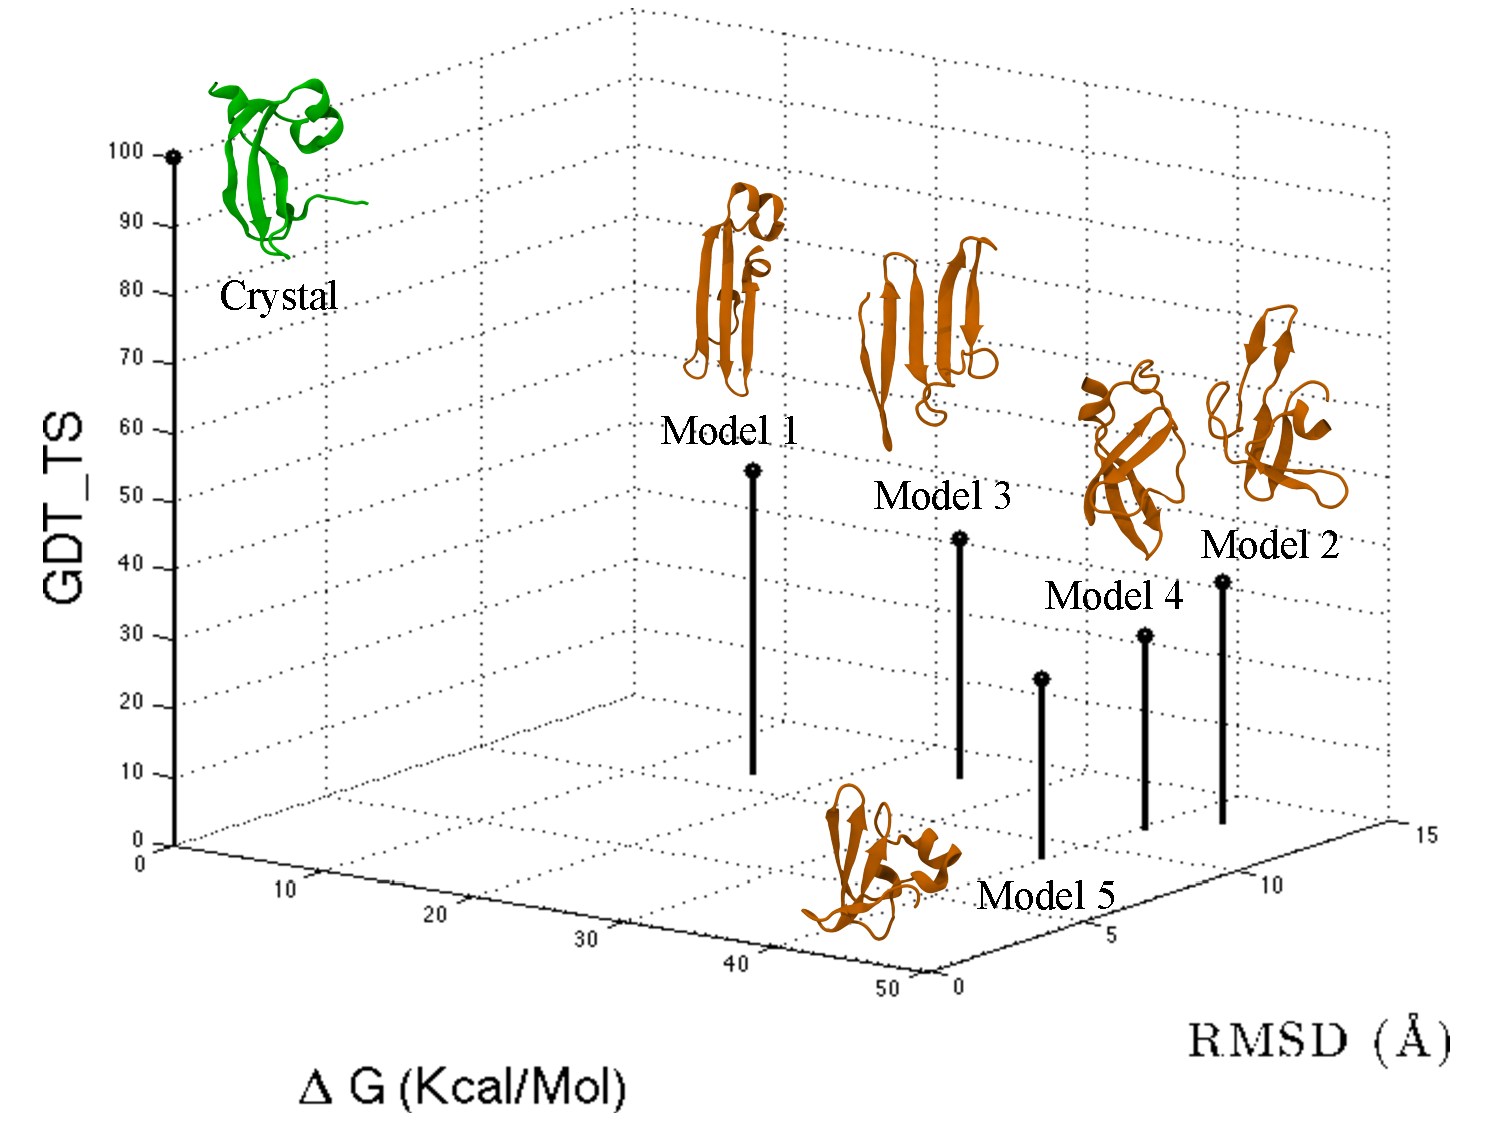
\includegraphics[width=3.5 in]{T0531.pdf}
\end{center}
\caption{The native structure and 5 models of extracellular domain of the jumping translocation breakpoint protein (pdb
    id: 2KJX and the CASP code: T0531).}
\label{fig:T0531}
\end{figure}


\begin{thebibliography}{99}

\bibitem{Krivov2009}
Krivov, G.G.; Shapovalov, M.V.; Dunbrack, RL Jr. Improved prediction of protein side-chain conformations with SCWRL4.
Proteins. (2009) 77, 778-795.

\bibitem{Perez2012}
Perez, A.; Yang, Z.; Bahar, I.; Dill, K.A.; MacCallum, J.L.; FlexE: Using Elastic Network Models to Compare Models of Protein Structure. J. Chem. Theory Comput., 2012, 8, 3985-3991.

\end{thebibliography}

%\end{suppinfo}
\end{document}
